\documentclass[12pt]{article}

\usepackage{amsmath}
\usepackage{amsfonts}
\usepackage{amssymb}
\usepackage[hmargin=1.5cm,vmargin=1.5cm]{geometry}
\usepackage[super,comma,sort&compress, square]{natbib}
\usepackage{graphicx}
\usepackage{tikz}
\usepackage{pgfplots}
\usepackage{float}
\usepackage{csvsimple}
\usepackage{gnuplottex}
\usepackage{todonotes}
\usepackage{csquotes}
\usepackage{pgfkeys}
\usepackage{listings}
\pgfplotsset{compat=1.7}
\usepackage[english]{babel}
\pgfplotsset{every axis y label/.append style={xshift=1.0em}}

\usepackage{hyperref} %% to turn the links clickable and load this before cleveref
\usepackage{cleveref}
\crefname{table}{table}{tables}
\Crefname{table}{Table}{Tables}
\crefname{figure}{figure}{figures}
\Crefname{figure}{Figure}{Figures}
\crefname{equation}{equation}{equations}
\Crefname{Equation}{Equation}{Equation}



\setlength\parindent{0pt} % Removes all indentation from paragraphs

%----------------------------------------------------------------------------------------
%	CODE INCLUSION CONFIGURATION
%----------------------------------------------------------------------------------------

\definecolor{MyDarkGreen}{rgb}{0.0,0.4,0.0} % This is the color used for comments
\lstloadlanguages{Perl} % Load Perl syntax for listings, for a list of other languages supported see: ftp://ftp.tex.ac.uk/tex-archive/macros/latex/contrib/listings/listings.pdf
\lstset{language=Perl, % Use Perl in this example
        frame=single, % Single frame around code
        basicstyle=\small\ttfamily, % Use small true type font
        keywordstyle=[1]\color{Blue}\bf, % Perl functions bold and blue
        keywordstyle=[2]\color{Purple}, % Perl function arguments purple
        keywordstyle=[3]\color{Blue}\underbar, % Custom functions underlined and blue
        identifierstyle=, % Nothing special about identifiers                                         
        commentstyle=\usefont{T1}{pcr}{m}{sl}\color{MyDarkGreen}\small, % Comments small dark green courier font
        stringstyle=\color{Purple}, % Strings are purple
        showstringspaces=false, % Don't put marks in string spaces
        tabsize=5, % 5 spaces per tab
        %
        % Put standard Perl functions not included in the default language here
        morekeywords={rand},
        %
        % Put Perl function parameters here
        morekeywords=[2]{on, off, interp},
        %
        % Put user defined functions here
        morekeywords=[3]{test},
       	%
        morecomment=[l][\color{Blue}]{...}, % Line continuation (...) like blue comment
        numbers=left, % Line numbers on left
        firstnumber=1, % Line numbers start with line 1
        numberstyle=\tiny\color{Blue}, % Line numbers are blue and small
        stepnumber=5 % Line numbers go in steps of 5
}

% Creates a new command to include a perl script, the first parameter is the filename of the script (without .pl), the second parameter is the caption
\newcommand{\java}[2]{
\begin{itemize}
\item[]\lstinputlisting[caption=#2,label=#1]{#1.pl}
\end{itemize}
}


\title{The Determination of a Value for the Newtonian Gravitational Constant, G with an Experimental Result from a Torsion Pendulum}
\author{Magdalen Berns
\\
s0946936 \\}
\date{\today}

\begin{document}
\maketitle
\thispagestyle{empty}

\begin{abstract}
\noindent
Here it has been used to learn t using the Acceleration Method. ThiThe period of the pendulum was determined to be 608(7) seconds (s). 

The gravitational constant was determined to be bla.... It was found that the error.
 \end{abstract}

\clearpage
\tableofcontents
\thispagestyle{empty}
\clearpage

\section{Introduction}

\subsection{Historical Background}

This experiment is a reproduction of the one performed by Henry Cavendish when he wished to determine the density of the earth using a torsion pendulum. The universal gravitational constant G, is not something that is easy to determine. The reason for this is that the earth is accelerating and it's gravitational force, $g$ is much greater than the literature value for G (or indeed, the value for G that Isaac Newton hypothesised in his book, Principia. Where here stated in theorem | that the force between two masses can be determined by the inverse of the distance between them. But, not without some gravitational constant! 


\subsection{Theory}

According to Isaac Newton, the force between two masses can be expressed as \cref{eq:grav}

\begin{equation}
\label{eq:grav}
\mathrm{F=\frac{G m_{1} m_{2}}{r^{2}}}
\end{equation}
\noindent 
Where $m_{1}$ and $m_{2}$ are masses and G. This equation is used to determine the mass of planetary systems 

\noindent 
Such a system as shown in \cref{eq:eom}, where damping is neglected.

\begin{equation}
\label{eq:eom}
\mathrm{I\frac{d^2\theta}{dt^2}+ \kappa\theta = 0}
\end{equation}
\noindent 
If we rearrange we can get an expression for the torque, $\tau$ under which a torsion pendulum acts.

\begin{equation} 
\label{eq:torque}
\mathrm{\tau =I\frac{d^2\theta}{dt^2}= -\kappa \theta}
\end{equation}

\noindent 
Solving \cref{eq:torque} allows us to see why the torsion pendulum oscillates at a frequency given by \cref{eq:resonant}

\begin{equation}
\label{eq:resonant}
\omega_n =\sqrt{\frac{\kappa}{I}}\,
\end{equation}
\begin{equation}
\label{eq:period}
\mathrm{T= \frac{2\pi}{\omega_n} = 2\pi \sqrt{\frac{I}{\kappa}}}
\end{equation}

\noindent
The glass is there in order to protect the small dumbbells from being disturbed by fluctuations in the air but because it is between the mirror and the detector, there is the issue of how the glass affects the path of the light to consider. This is because the principle of moments, expressed in \cref{eq:moments} indicates that the forces in the local vicinity of the dumbbells will have an effect on their oscillatory motion.  

\begin{equation}
\label{eq:moments}
\mathbf{r}\times\mathbf{F}_1 + \mathbf{r}\times\mathbf{F}_2 + \cdots = \mathbf{r}\times(\mathbf{F}_1+\mathbf{F}_2 + \cdots  +\mathbf{F}_n )
\end{equation}

\noindent 
Where $r$ is the position vector and it is perpendicular to the Force, F. 


\noindent 
It is possible to perform a small angle approximation so that $\mathrm{sin}\left(\frac{\delta}{2}\right)\approx\left(\frac{\delta}{2}\right)$. Since $\delta$ can be determined from the distance, $\Delta S$ found by the separation between the equilibrium of the pendulum when it is subjected to torsion from one side until it reaches equilibrium and then subjected to the other side as expressed in \cref{eq:delta}. The angle made by the reflected light wave given by \cref{eq:deltafin} with $R$ being the coefficient of reflectivity. 

\begin{equation}
\label{eq:deltaS}
\mathrm{\Delta S = S_{1}-S_{2}}
\end{equation}


\section{Experimental Method}

Two balls, each of mass $0.015\mathrm{kg}$ were separated by a small rigid rod suspended $\approx$ 26cm from a wire string from their centre of mass (CoM) inside a circular case with glass faces on either side. It was necessary to suspend the from a height. This was done using a thin copper cable so that the diamagnetic properties of the copper would prevent it from becoming magnetised. with enough torsion to before the pendulum could 

\subsection{Equipment}


%%%%%%%%%%%%%%%%%%%%%%
%
%           Figure 
%
%%%%%%%%%%%%%%%%%%%%%%

\begin{figure}[H]
\centering
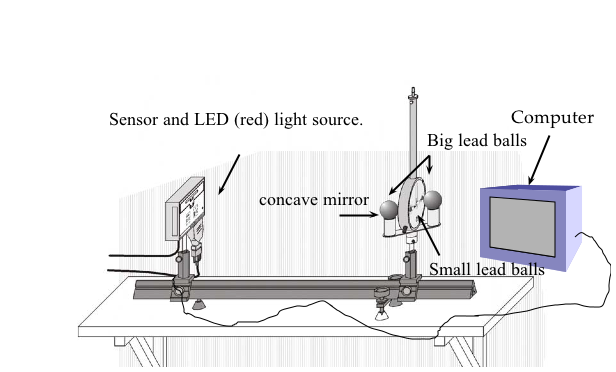
\includegraphics[width=15cm, height=10cm]{images/schematic.png}
\caption{A Schematic of the Cavendish}
\label{fig:probe}
\end{figure}

The torsion band was a brass wire with a torsion constant of approximately $ 8.5 \times{10^{-9}}\mathrm{Nm/rad }$

\subsection{Preparation and Calibration}

Before anything, the system had to be calibrated to zero point. This was because the periodic motion of the pendulum was highly sensitive to the initial conditions. Initially the pendulum torsion band had become slack. It took several days of calibration to solve this. The torsion band was so delicate is snapped and the head had to be replaced, while the torsion band was sent for repair. The experiment continued with a newly calibrated set up.

The core experimental apparatus comprised of two lead masses each weighing $0.015(5)\mathrm{kg}$, each with a diameter 13.0(1)mm which were screwed fast at both ends to make a set of tiny dumbbells of length 111.7(1)mm, a case to keep them in, two larger balls of mass $1.508(2)\mathrm{kg}$ and $1.509(2)\mathrm{kg}$, an electronic light sensor, 

The dumbbells were then attached to a special brass wire called a torsion band which was held fast by a knurled knob so it could be suspended from a height of $\approx 260\mathrm{mm}$ (according to the laboratory manual).  The dumbbells were kept inside a protective housing with glass windows at either side and this was positioned parallel to their length. The pendulum was then calibrated so that the dumbbells were able to hang freely about their centre of mass with a concave mirror attached to their \enquote{front} so that a sensor positioned $L=648.7\mathrm{mm}$, which was emitting light from two light emitting diodes (LEDs), would pick up the reflected, polarised beams and convert this result to a digital signal in order to run it on some provided propeitry software called \enquote{CASSY Labs} for analysis.

Because the motion of the dumbbells was so easily disturbed it needed to be left overnight to settle to equilibrium and then were positions on two ball holders and gently swivelled so that they were touching the glass without knocking the dumbbells. This provided a torsion which would be just enough to displace the dumbbells from equilibrium, without knocking the case. The dumbbells were again left so that their oscillations could decay and the resulting signal converged to a position $S_{1}$. Once the was a clear sign that the signal had settled in one position, $S_{1}$ the larger balls were swivelled so that they would touch the glass on the other side, applying a torsion there without knocking the dumbbells to a chaotic motion. This allowed the motion of the dumbbells to settle to a position $S_{2}$

The difference between the two positions of equilibrium would give vital information about the angle the displaced dumbbells made with respect to the sensor which faced their equilibrium at a distance L, directly in front of them. This is expressed mathematically in \cref{eq:theta}.

\begin{equation}
\label{eq:theta}
\mathrm{\theta = \frac{\Delta S }{4L}}
\end{equation}

 

The angle was as a result of the force from the mass of the balls on the ball holders which were made to apply a torsion to displace the dumbbells so that they oscillated until the reached equilibrium with a bias to one side. At this stage when the signal indicated the motion had reached equilibrium, the balls were again swivelled to rest at the opposite side thus applying a torsion there. 

Once this had completed the remaining measurements were made, to determine any errors which may have been missed when trying to keep the system from being disturbed. Some corrections were made and the system was allowed to settle in an attempt to improve increase the precision of results and the first set of data were calculated to determine value for G. 

The distance  $\Delta S$ was qualitatively determined first by running the CASSY Lab software to get the value for a mouse pointer determined distance between the two converged points displayed on the file. The software was then run to obtain an envelope result to try and assertion whether this would give a better estimate of the $\Delta S$. Ultimately the software was converted to ASCII so that a mean of the convergent data points could be calculated and compared with the CASSY Lab estimations using a java program designed for data analysis\cite{me}. It was determined that the latter method was more reliable as the result was within the 2$\%$ precision and since this was estimate of the hardware analogue to digital conversion of the sensor equipment  obtained from the PASCO manual provided.

A calculation of period based on the given value for torsion of the wire as given from the information in the data sheet then we would expect the period to be \todo{bla} from \cref{eq:Time}. If we use the oscillations printed to the ASCII  file by the computer software  
\section*{Corrections}
The coherence of a red LED is typically 0.4.\cite{red} which is fairly low. However the pendulum was set up so that the LED would shine only  655.1(2)mm away from the This meant that 
\begin{equation}
\label{eq:Time}
\mathrm{T = \frac{4\pi^2 I}{\kappa}}
\end{equation}
%%%%%%%%%%%%%%%%%%%%%%
%
%           Map
%
%%%%%%%%%%%%%%%%%%%%%%


\begin{figure}[H]
\centering
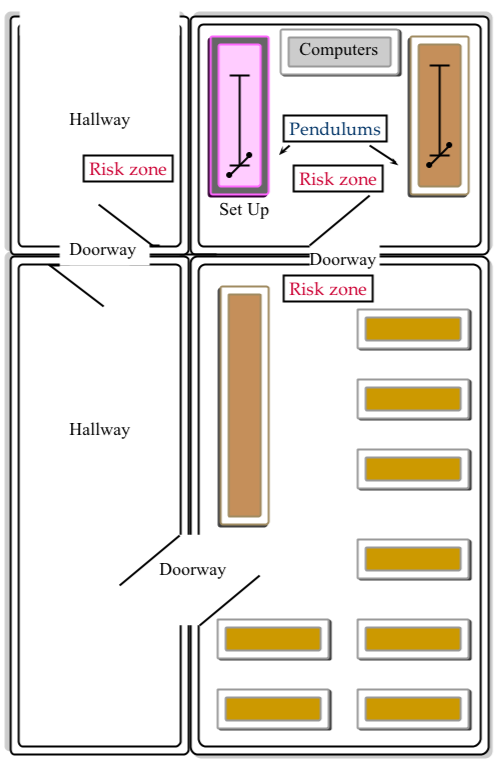
\includegraphics[width=8cm, height=11cm]{images/map.png}
\caption{A map of the local vicinity of the experiment. The experiment site is indicated in the pink table along with the high risk zones because it is through the double doors were a lot of activity from people moving through the doorway would cause the walls to shake which was likely to lead to chaotic fluctuations in the pendulum}
\label{fig:probe}
\end{figure}

%%%%%%%%%%%%%%%%%%%%%%
%
%           Acceleration
%
%%%%%%%%%%%%%%%%%%%%%%

\subsection{Acceleration Method}

According to the manual

%%%%%%%%%%%%%%%%%%%%%%
%
%           BY Equilibrium Positions
%
%%%%%%%%%%%%%%%%%%%%%%


\section{Measurement by Equilibrium Positions}


According to the manual this was expected to give the most accurate result when compared with the literature value.

%%%%%%%%%%%%%%%%%%%%%%
%
%           End Deflection
%
%%%%%%%%%%%%%%%%%%%%%%

\subsection{End-deflection Method}


\begin{equation}
\label{eq:gdef}
\mathrm{G=\frac{\pi^{2}\Delta{S} d b }{T^{2}m_{1}L}}
\end{equation}


The value for $\Delta{S}$ was $18.7(2)\mathrm{m}$. This lead to a value for the angle as being. The trickiest part of ascertaining a value for the period. The reasons for this will be discussed with the results.  This is because the oscillations gave different result for each different peak to peak measurement. This was likely not to have been due to the A/D conversion because the resolution of the equipment was only 1\%.

The error in $T^{2}$ was determined using \cref{eq:errort} so that the 

Finally, the errors were combined to obtain a result for G 

\begin{equation}
\label{eq:errors}
\mathrm{\sigma=\sqrt{\left(\frac{\Delta L }{L}\right)^{2}+\left(\frac{\Delta b}{b}\right)^{2}}}
\end{equation}

\section{Results and Discussion}

\subsection{Limitations of the Experimental Method and Future Consideration}

Although stationary walls cannot affect the forces acting on the masses in principle. The walls are not completely stationary when there are people walking about or banging outside, the noise is heard through the walls this is because the oscillations from sound waves travelling around in the walls which could have potentially affected the table. The action of swivelling the balls should ideally be friction free and smooth but in reality it required a steady hand and because of the diverse motion of the human arm and hand, is also not very reproducible. Therefore this experiment could be greatly improved by using a mechanical arm to swivel the mass. That way the arm could be configured to repeat the same motion in the same way every time. 

The experiment could also be improved by placing the pendulum on a solid marble table. This would prevent the set up from being accidentally knocked. It could also be possible that tmtion in the corridor as a worse affect on t

%%%%%%%%%%%%%%%%%%%%%%
%
%           Conclusion
%
%%%%%%%%%%%%%%%%%%%%%%

\section{Conclusion}

%%%%%%%%%%%%%%%%%%%%%%
%
%           Acknowledgements 
%
%%%%%%%%%%%%%%%%%%%%%%

\bibliography{pendulum}
\bibliographystyle{unsrt}


\section{Acknowledgements}

\section{Appendix}

\begin{table}[htdp]
\vline
\begin{tabular}{| r | c | r  | c | r  | c | r |  c | r }
\hline 
Variable & L & b & d  & $\Delta S$  \\
Tool & meter rule  & calliper  & calliper & CASSY Lab   \\
Value  &  &  &  &  &   \\
Error &  &  &  &  &   \\

\end{tabular}
\vline
\caption{A table of measured values }
\end{table}%

\begin{center}
\begin{table}[H]
\centering
\begin{tabular}{| r | c | r  | c  | | r  | } 
\hline


& Diameter $\mathrm{m_{2}}$ & Variance  \\
\hline
mass, $m_{2_{a}}$ & 63.6 & 0.3481  \\
& 61.3 & 2.924 \\
& 63.3 & 0.0841 \\
& 63.8 & 0.6241 \\
& 63.9 & 0.9721 \\
\hline
mass, $m_{2_{b}}$  & 61.5 & 2.2801 \\
& 63.5 & 0.2401 \\
& 63.6 & 0.3841 \\
& 63.6 &  0.3841 \\
& 62.0 & 1.0201 \\
\hline 
mean & 60.01 &  \\
\hline
std deviation & & 0.949 \\
\hline
\end{tabular}
\caption{A table of measured values for the diameter of the large balls, $m_{2}$. For each ball, five values were recorded using the digital calliper and  }
\end{table}%

\end{center}





\end{document}